% !TEX root = template.tex

\section{Processing Pipeline}
\label{sec:processing_architecture}

\begin{figure*}[h]
	\centering
	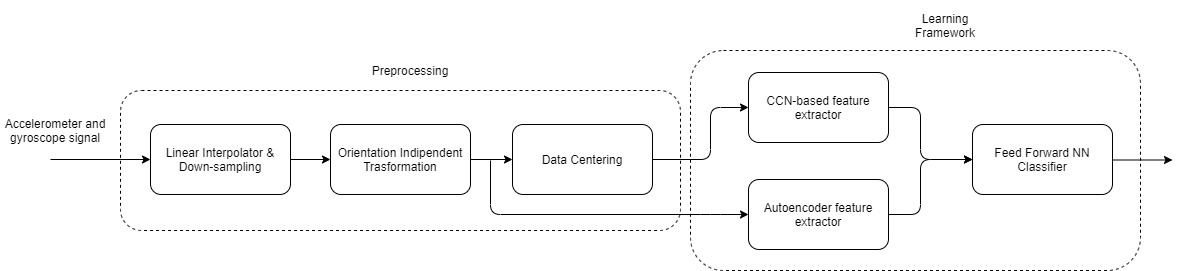
\includegraphics[width=1\textwidth]{images/processing_pipeline.jpg}
	\caption{Processing pipeline}
\end{figure*}

The task of HAR in real use case scenarios is a difficult task, and many aspects need to be considered when these applications are brought in a mobile environment. As reported in \cite{blunck2013heterogeneity} the three major types of heterogeneties which yield impairments in HAR are:
\begin{itemize}
	\item \textbf{Sensor Biases}: To keep the overall cost of a smartphone low, low costs accelerometer and gyroscope sensor are used, yielding a poor-calibrated, inaccurate an of limited granularity and range acquired signals. So, among this type of sensors we could observe differences in precision, resolution, range and also biases. Usually an initial sensors calibration are made by smartphones manufactures, but due to rotation or misalignment of the sensor to the circuit board of the final product, this could introduce errors. Furthermore, if a device experience shock, e.g falling on the ground, the sensor can be misaligned causing unwanted biases.
	\item \textbf{Sampling Rate Heterogeneity}: Often popular smartphones vary in terms of the default and supported sampling frequencies for accelerometer and gyroscope sensor. In the dataset TODO riportare link used for this experiment for example we are dealing with smartphone where the sampling frequency varies from 50Hz to 200Hz. See Fig. TODO so the actual number of devices used in this dataset, with their corresponding sampling frequencies.
	\item \textbf{Sampling Rate Instability}: This phenomenon is specific to a single device and regards the regularity of time span between successive measurements. Different factors could accentuate this problem, including heavy multitasking or high I/O load in the mobile device. Multitasking effect in particular is a major problem: smartphone usually prioritizes among various running tasks and doing so could extremely affects the sensor sampling of a HAR application running on the device. In our collected dataset with a 100 Hz sampling rate,for example we observe a time span between consecutive measurement of TODO, even if the smartphone was hold in \textit{airplane mode} to reduce at the minimum this effect. The Fig. TODO shows the amount of different time-span present in our dataset.
\end{itemize}

Furthermore, if we considered a real use case scenarios of a HAR mobile application we must also consider that smartphones can be positioned and oriented in different ways in human body. For example a smartphone could lay in trouser pockets (back and front) or maybe inside accessories like in a pouch or in a bag with different orientations. These different initial model settings have huge effects in prediction accuracy of an HAR predictor, especially if the model has been trained on a dataset that consist of activity measurement coming from only one fixed position and orientation of the smartphone, as is usually the case dealing with dataset collected in a controlled environment that could be found on Internet. 

To tackle all these problems we decided to adopt in our pre-processing pipeline as show in Fig. TODO, 3 main blocks.

The first block called Linear Interpolator is in charge of mitigate the problems regarding the Sampling Rate Heterogeneity and Sampling Rate Instabilities as discussed previously. It main purpose is to down-sample the input data to a fixed sampling rate, in our case 50 samples/second. 

The second block called Orientation Independent Transformation is used to represent data coming from different orientation of the smartphone in a rotation independent space. In this way all the signals are projected in a new space whose orientation is independent of that of the smartphone and aligned with gravity and the direction of motion. In this way an user can place his smartphone in whatever position he or she wants, mitigating the problem of different position and rotations of smartphone, as we will see in the Experiment section TODO reference.

Our last block consists of a data centering operation, applied for centering signals among y-axis that are presented only for the Covolutional Layer and not for the Autoencoder block. The reason of this choice would be clear in the section TODO. As reported in \cite{ignatov2018real}, time series centering standardize the input data, making the task for the CNN easier. Data normalization instead must be avoided because does not help in this situation since it significantly distorts time series shape, removing magnitude information which is critical for activities differentiation.

After the preprocessing pipeline we adopt a novel Learning framework. It is composed of CNN augmented with features coming from an autoencoder. As discussed in \cite{ignatov2018real} CNNs learns filters that are applied to small sub-regions of the data, and therefore they are able to capture local data pattern and their variations. Additionally, due to a small number of connections and high parallelism the amount of computations and running time of CNNs is significantly lower compared to other deep learning algorithm. This yield these model perfect for real-time HAR apps, where these models could also run in a restrict environment as one like smartphones where computation resources are limited. The only drawback of CCNs is that they fall behind in capturing global properties of the signal, and as proposed in \cite{ignatov2018real} they resolve this problem by augmenting CNNs with some basic statistical features that comprise this aspects of the data. But as opposed to what done in this latter work, where they used manual extracted features, we decided to opt for a autoencoder features extractors which can provide more robust feature. For this reason we train an auto-encoder separately on the training data and then use the encoder part to augment the CNN features used for the last classification Feed Forward Neural Network. 

\section{Signals and Features}
\label{sec:model}

Parlare del nostro dataset usato Heterogenity, cioe come sono strutturati i nostri dati partenza. 



\subsection{Dataset \& Meausurement Setup}
Parlare di come abbiamo splittato il dataset, quindi escludendo gli utenti a e b per fare in modo di testare le performance cambiando compltamente utente.

Introduzione e spiegazione del dataset eterogeneo, preso da: riportare link. e riportare come abbiamo tirato fuori le time window con overlapping window!

Accenare dell'acquisizione di un nostro dataset alla stessa maniera, a 100 HZ in varie posizioni per testare poi anche tutto il dataset!

\subsection{Signal preprocessing}

In questo caso si va nel dettaglio (con formule e forse se neccessario anche grafici) della parte di preprocessing (parte trattegiata nel mio schema come preprocessing):

\textbf{Notation}: With $\boldsymbol{x}$ we mean a column vector $\boldsymbol{x}=(x_{1}, x_{2}, ..., x_{n})^{T}$.  With $\boldsymbol{||x||}$ we mean the L2-norm operator and with $\bar{x} = \sum_{i=1}^{n} x_{i} / n$ the mean of a vector. With $\boldsymbol{x} \cdot \boldsymbol{y} =\boldsymbol{x}^{T}\boldsymbol{y} $ we mean the inner product of two vectors. With $\boldsymbol{\vec{x}}$ we mean a 3D vector $\boldsymbol{\vec{x}} = (x_{1}, x_{2}, x_{3})^{T}$ and with $\boldsymbol{\hat{x}}$ the corresponding 3D versor $\boldsymbol{\hat{x}}=\boldsymbol{\vec{x}}/ ||\boldsymbol{\vec{x}}||$. For any two 3D vector $\boldsymbol{\vec{x}}$ and $\boldsymbol{\vec{y}}$ we indicate their cross-product as $\boldsymbol{\vec{x}} \times \boldsymbol{\vec{y}}$. We represent with $\boldsymbol{a_{x}}, \boldsymbol{a_{y}}, \boldsymbol{a_{z}}$ the x, y and z components of the accellerometer signal, as well as the gyroscope signal is represented with $\boldsymbol{g_{x}}, \boldsymbol{g_{y}}, \boldsymbol{g_{z}}$. We define also matrices with uppercase and bold letters. For example to define a $3 \times n$ matrix composed of 3 vectors $\boldsymbol{x}, \boldsymbol{y}, \boldsymbol{z} \in {\rm I\!R}^{n}$ we use the notation $\boldsymbol{M} = [\boldsymbol{x}, \boldsymbol{y}, \boldsymbol{z}]^{T}$\\

\textbf{Linear Interpolation \& Down-sampling}\\

\textbf{Orientation Indipendent Transform}\\
To project the signals acquired during an activity in a new space wich is indipendent of the rotation of the smartphone, 3 orthogonal versors need to be found. We decided to adopt the technique proposed in \cite{gadaleta2018idnet}, although many other works proposed a similar solution as in \cite{kunze2009way, henpraserttae2011accurate}. In summary we have to find these 3 orthogonal versor namely vertical versor $\boldsymbol{\hat{v}}$, horizontal versor $\boldsymbol{\hat{h}}$ and lateral versor $\boldsymbol{\hat{l}}$. As the name suggest the vertical versor is aligned with user torso pointing up, the horizontal versor is aligned with the direction of motion, pointing foraward, and the later versor tracks lateral movements and it is othogonal to the other two.

Starting with the vertical versor we need to find where the gravity vector $\boldsymbol{\vec{p}}$ ly in the original space. Although the gravity vector is a constant vector in stationary conditions, during a user activity it continuosly changes in the original cordinate system of the smartphone, therefore we are only able to consider the mean direction of the gravity within the current user activity. So, to estimate it we must considered only the acceleremoter signal: $ \boldsymbol{\vec{p}} = (\bar{a_{x}}, \bar{a_{y}}, \bar{a_{z}})^{T}$  and we now could find the vertical versor with $ \boldsymbol{\hat{v}} = \boldsymbol{\vec{p}} / ||\boldsymbol{\vec{p}}|| $ 

This is the first axis of our new space, and we can project the datas onto this new versor to obtain the first component axis. To do we define the acceleration matrix $\boldsymbol{A} = [ \boldsymbol{a_{x}}, \boldsymbol{a_{y}}, \boldsymbol{a_{z}} ]^{T}$ and the gyroscope matrix $\boldsymbol{G} = [ \boldsymbol{g_{x}}, \boldsymbol{g_{y}}, \boldsymbol{g_{z}} ]^{T} $. Now we could project the data onto $\boldsymbol{\hat{v}}$ by:

$$ \boldsymbol{a_{v}} = \boldsymbol{A} \cdot \boldsymbol{\hat{v}} ,\;\; \boldsymbol{g_{v}} = \boldsymbol{G} \cdot \boldsymbol{\hat{v}} $$

Now we have to find an horizontal plane, parallel to the floor, where the activity motion mostly occurs. To do so we have to remove the  $\boldsymbol{a_{v}}$ component from the original data. We represent the accelerometer data lying on this new plane as $\boldsymbol{M}$ representing the so called motion plane. To find $\boldsymbol{M}$ we have to: $\boldsymbol{M} = \boldsymbol{A} - \boldsymbol{\hat{v}} \boldsymbol{a_{v}}^{T} $

In this new plane, we could see that the direction with the largest variance of projected data, represents the main direction of motion, ie in which direction the user is currently performing the activity with respect to the current smartphone orientation. By aplying PCA \cite{rao1964use}, we are able to find the direction along which the variance of measurements is maximized. This new extracted vector it is called horizantal vector $\boldsymbol{\vec{h}}$. We now could compute the horizontal versor:	$ \boldsymbol{\hat{h}} = \boldsymbol{\vec{h}} / ||\boldsymbol{\vec{h}}|| $ and we are now able to project our data onto this second new axis by:

$$ \boldsymbol{a_{h}} = \boldsymbol{A} \cdot \boldsymbol{\hat{h}} , \;\; \boldsymbol{g_{v}} = \boldsymbol{G} \cdot \boldsymbol{\hat{h}} $$

To find the last axis its sufficient to apply a cross product between the two last axis found, so $ \boldsymbol{\hat{l}} = \boldsymbol{\hat{v}} \times \boldsymbol{\hat{h}} $ and the obtain our last projection of the original data into this new space by:

$$ \boldsymbol{a_{l}} = \boldsymbol{A} \cdot \boldsymbol{\hat{l}} , \;\; \boldsymbol{g_{l}} = \boldsymbol{G} \cdot \boldsymbol{\hat{l}} $$

Our final accelerometer and gyroscope trasformed vectors lying in this new orientation indipendent space is $(\boldsymbol{a_{v}}, \boldsymbol{a_{h}}, \boldsymbol{a_{l}}) $ and $ (\boldsymbol{g_{v}}, \boldsymbol{g_{h}}, \boldsymbol{g_{l}}) $ \\

\textbf{Centering}\\
	

\begin{itemize}
	\item interpolazione lineare / downsampling
	\item rotational invariant citare tutti i paper e come funziona
	\item centering
\end{itemize}

\subsection{Feature vector}
\begin{itemize}
	\item window strategy
	\item basic feature extraction
	\item autoencoder feature extraction
\end{itemize}

\section{Learning Framework}
\label{sec:learning_framework}

\begin{figure*}[h]
	\centering
	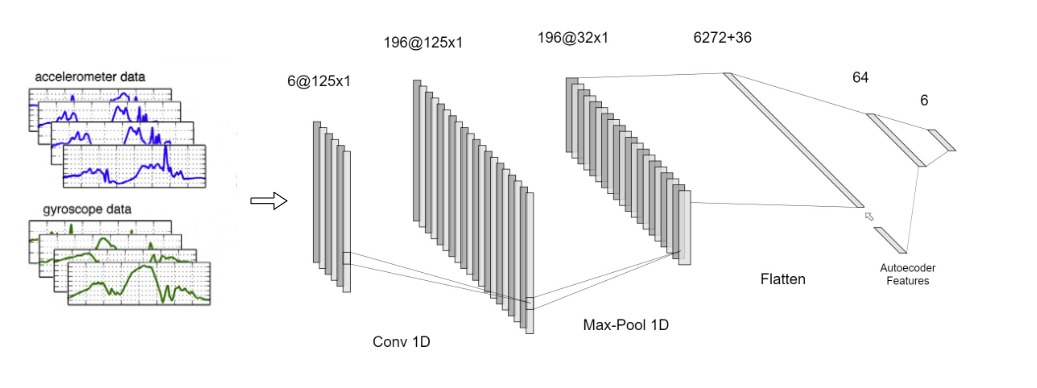
\includegraphics[width=1\textwidth]{images/full_architecture.jpg}
	\caption{Learning Framework}
\end{figure*}

Desctivere qui invece la parte tratteggiata come learning framework

Descivere prima l'autoencoder, come è stato costruito e come viene allenato. TODO luca

Passare alla decrizione della mia archittetura, come sono stai selezionati gli iper-parametri, ecc ecc.

